\documentclass[../main.tex]{subfiles}
\graphicspath{{img/}}
\begin{comment}
    Materials, apparatus, and procedures. List and describe key materials and apparatus. Then describe the procedure in enough detail that others can duplicate it. For design studies, this section includes component design, fabrication, assembly, and testing procedures. Use illustrations.

    Results. Present the results, usually with accompanying tables and graphs. Characterize the patterns and quality of the results and estimate their accuracy and precision. Detailed data go to an appendix. Use analytical graphics.
\end{comment}

\begin{document}
\section{Trigger \emph{TrigFromBeam}}
%intro della section, problema fisico
I raggi cosmici sono una fonte naturale di particelle cariche ad alta energia che, interagendo con l'atmosfera, giungono alla superficie terrestre. Tutti gli esperimenti che utilizzano rilevatori di particelle cariche presentano un segnale di fondo generato dalla presenza di raggi cosmici. In alcuni casi questo può minacciare la riuscita dell'esperimento, per esempio nel caso si voglia rilevare eventi meno energetici e rari come i neutrini \cite{cosmicrays}.
A seconda delle caratteristiche dell'esperimento e del fenomeno fisico di interesse, è possibile simulare questo segnale di fondo per poi andare a rimuoverlo. Altrimenti è possibile sviluppare algoritmi di identificazione degli eventi generati dai raggi cosmici.

Si presenta l'algoritmo di identificazione di eventi generati da raggi cosmici sviluppato per il prototipo di rilevatore descritto nel capitolo precedente (matrice $3 \times 3$ di calorimetri e fotomoltiplicatori). L'acquisizione dati è gestita da TriDAS e l'algoritmo è inserito come \emph{trigger} L2.
%algoritmo
Per prima cosa si mostra l'interfaccia definita da TriDAS per un trigger L2.
Il trigger L2 ( o \emph{trigger plugin}), in questo caso \emph{TrigFromBeam}, è dichiarato come una funzione che prende come argomento un oggetto di tipo \emph{PluginArgs} 
\begin{lstlisting}[language=C++,frame=none]
void TrigFromBeam(PluginArgs const& args);
\end{lstlisting}
con
\begin{lstlisting}[language=C++,frame=none]
struct PluginArgs
{
  int id;
  EventCollector* evc;
  Geometry const* geom;
  Configuration const* params;
};
\end{lstlisting}
Quindi l'algoritmo dispone degli eventi appartenenti a una certa \emph{TimeSlice} (TS), della geometria dell'apparato e del file di configurazione fornito dall'utente.
Per ciascun evento della TS, l'algoritmo riempie un vettore chiamato \texttt{seeds} con le \emph{hit}, i.e. picchi di segnale, selezionate dal \emph{trigger} L1, dette \emph{seed} del \emph{trigger}.
\lstinputlisting[linerange={181-181},language=C++,frame=none]{../lst/TrigFromBeam/TrigFromBeam.cpp}
Infatti l'energia media di un muone cosmico alla superficie terrestre ($\small\sim$\SI{4}{GeV}) è tale da superare la soglia del trigger L1 (\SI{2}{GeV}).
Le \emph{hit} sono rappresentate dal tipo \texttt{PMTHit}, che contiene l'indice identificativo del sensore che ha prodotto la \emph{hit}, il tempo di arrivo, la carica elettrica del picco di segnale, etc. 
Quindi, per ciascun \emph{seed} \texttt{this\_seed} del vettore \texttt{seeds}, si verifica la presenza di altri \emph{seed} correlati spazio-temporalmente a \texttt{this\_seed}. In caso affermativo, i \emph{seed} corrispondenti sono inseriti in un vettore chiamato \texttt{cosmic\_trace}.
\lstinputlisting[language=C++,frame=none,emph={[3]this_seed},emphstyle={[3]\color{blue}},caption={Algoritmo di selezione di \emph{hit} generate da raggi cosmici implementato dalla funzione \texttt{TrigFromBeam}.},label={lst:algo}]{../lst/algo_short.cpp}
La correlazione spaziale e temporale dipende dalla geometria dell'apparato e dal fenomeno fisico in questione. Nel caso dei raggi cosmici, possiamo considerare in prima approssimazione muoni che volano in direzione perpendicolare alla superficie terrestre a velocità prossime a $c$. 
L'apparato del rilevatore è il prototipo descritto nel capitolo precedente (\autoref{sct:jlab}). Consideriamo quindi una matrice $3 \times 3$ di rilevatori, ciascuno di sezione quadrata di lato $d$.
Quindi, nel caso di passaggio di un muone cosmico all'interno del rilevatore, ci aspettiamo di trovare \emph{hit} successive in una colonna di rilevatori, a distanza temporale di $\small\sim\frac{d}{c}$.

La correlazione spaziale e temporale è definita dalle funzioni \texttt{timeCorrelation} e \texttt{spaceCorrelation}.
La funzione \texttt{timeCorrelation} prende come argomento due \emph{hit} e restituisce \texttt{vero} o \texttt{falso} a seconda che siano soddisfatti i criteri di correlazione temporale.
Per tenere conto di possibili variazioni statistiche del valore della velocità di volo e di traiettorie non propriamente verticali, la funzione verifica che la distanza temporale tra le due \emph{hit} cada all'interno di un intervallo.
La distanza temporale minima \texttt{shortest\_correlation\_time\_frame} tra due \emph{hit} è $\frac{d}{c}$, ovvero quella generata da un muone che cade perpendicolare alla superficie terrestre a velocità $c$.
La distanza temporale massima \texttt{longest\_correlation\_time\_frame} è definita come $\frac{\sqrt{2}d}{0.9\ c}$, ovvero quella tra due \emph{hit} generate da un muone che cade con inclinazione di $45^\circ$ rispetto alla superficie terrestre a velocità $0.9c$.

\lstinputlisting[linerange={118-124},language=C++,frame=none,caption={Algoritmo di correlazione temporale implementato dalla funzione \texttt{timeCorrelation}. L'unità di misura \texttt{fine\_time} corrisponde a \SI{e-9}{\s}.}]{../lst/TrigFromBeam/TrigFromBeam.cpp}

La funzione \texttt{spaceCorrelation}, analogamente alla precedente, prende come argomento due \emph{hit} e verifica i criteri di correlazione spaziale.
Sostanzialmente c'è correlazione quando la traiettoria tracciata dalle due hit è compatibile con un'inclinazione massima di $45^\circ$ rispetto alla verticale. Per controllare questa condizione si sfrutta la disposizione dei sensori all'interno della matrice.
Ciascuna \emph{hit} contiene l'indice del sensore che l'ha prodotta. I sensori sono identificati da indici crescenti, in questo caso da $0$ a $8$. Quindi l'algoritmo fa uso delle funzioni \texttt{row} e \texttt{col} per ottenere gli indici riga e colonna di ciascun sensore all'interno della matrice $3 \times 3$. Per esempio, il sensore con indice $6$ sarà il primo dell'ultima riga, ovvero indice riga $2$ e indice colonna $0$.
Ora, supponiamo che la \emph{hit} \texttt{this\_seed} sia prodotta dal sensore nella posizione \texttt{(1,0)} della matrice (\autoref{fig:3x3_sketch}). Le possibili traiettorie percorse da un muone cosmico per arrivare al sensore \texttt{(1,0)} attraversano il sensore soprastante \texttt{(0,0)} o uno di quelli adiacenti ai vertici \texttt{(0,1)}. Quelli sottostanti di conseguenza. 
Si tratta quindi di implementare una regola sugli indici in modo da selezionare i sensori corretti. Preso un elemento della matrice $e_{i,j}$, allora le due diagonali che lo comprendono sono definite da
\begin{equation}
	d_a = \{ e_{i',j'} \mid i' + j' = a\}
\end{equation}
e 
\begin{equation}
	d_b = \{ e_{i',j'} \mid i' - j' = b\}
\end{equation}
con 
\begin{equation}
a \coloneqq i + j \mathrm{,}\ b \coloneqq i - j
\end{equation}
Gli elementi soprastanti $e_{i,j}$ compresi tra le due diagonali $d_a$ e $d_b$ sono definiti da
\begin{equation}
	I_{up} = \{ e_{i',j'}\ \mid\ i' + j' \leq a\ \land\ i' - j' \leq b\}
\end{equation}
Gli elementi sottostanti $e_{i,j}$ compresi tra le due diagonali sono definiti da 
\begin{equation}
	I_{down} = \{ e_{i',j'}\ \mid\ i' + j' \geq a\ \land\ i' - j' \geq b\}
\end{equation}
Se un \emph{seed} è stato prodotto da un sensore la cui posizione appartiene all'insieme unione $I_{up}\ \cup\ I_{down}$, allora può essere correlato al seed \texttt{this\_seed}.
L'algoritmo verifica anche che una \emph{hit} prodotta da un sensore soprastante il sensore che ha prodotto \texttt{this\_seed}, sia precedente temporalmente a \texttt{this\_seed}. Analogamente, una \emph{hit} prodotta da un sensore sottostante il sensore che ha prodotto \emph{this\_seed}, deve essere anche successiva temporalmente a \texttt{this\_seed}.

\lstinputlisting[linerange={75-85},language=C++,frame=none,caption={Algoritmo di correlazione spaziale implementato dalla funzione \texttt{spaceCorrelation}.}]{../lst/TrigFromBeam/TrigFromBeam.cpp}

\begin{figure}[tb]
	\centering
	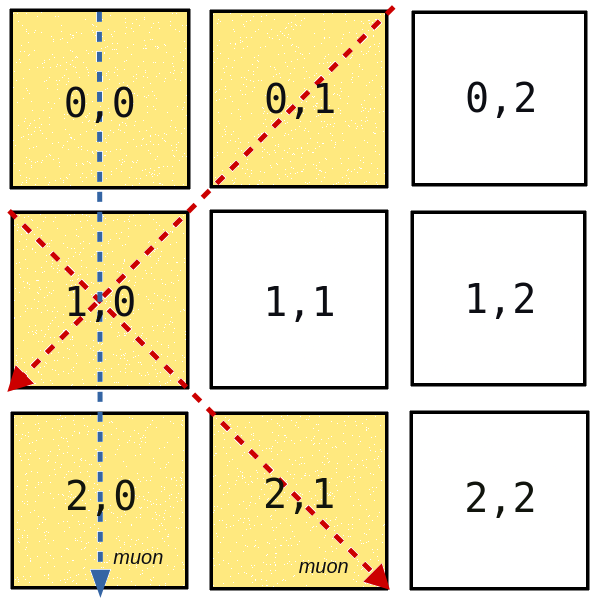
\includegraphics[width=0.5\textwidth]{3x3_side_indexes.png}
	\caption{Schema della sezione trasversale dell'apparato sperimentale. Le linee tratteggiate rosse e blu rappresentano le possibili traiettorie più lunghe e più corte rispettivamente con cui i muoni cosmici possono attraversare il sensore \texttt{(1,0)} dell'apparato, attivando di conseguenza i sensori indicati in giallo. All'interno di ciascun sensore sono indicati gli indici riga e colonna.}
	\label{fig:3x3_sketch}
\end{figure}

Infine, se un \emph{seed} non risulta correlato spazio-temporalmente con nessun altro \emph{seed} dell'evento significa che è stato prodotto da una particella del fascio, e viene quindi selezionato per essere salvato in memoria all'interno del PT file. 
Inoltre tramite la funzione \texttt{getParticleEnergy} viene calcolata la somma della carica del \emph{seed} con le cariche di tutte le \emph{hit} dello stesso evento distanti al più \SI{8}{\ns} dal \emph{seed}, fornendo così la carica totale dell'evento, proporzionale all'energia della particella.
%inserimento in TriDAS
%logica

Si vede come l'algoritmo sia strutturato in modo da sfruttare una logica generale tramite le funzioni \texttt{timeCorrelation} e \texttt{spaceCorrelation}, lasciando a queste l'implementazione dei criteri specifici di correlazione spazio-temporale per l'esperimento in questione. In questo modo si è cercato di rendere l'algoritmo il più possibile astratto e adattabile a diverse configurazioni dell'apparato sperimentale.

L'algoritmo fa uso del sistema di \emph{logging} \texttt{TRIDAS\_LOG} implementato in TriDAS per comunicare risultati e errori. 
\lstinputlisting[linerange={255-257},language=C++,frame=none,caption={Esempio di uso del sistema di \emph{log}. Prima di terminare l'esecuzione, viene riportato il numero di \emph{seed} selezionati dal \emph{trigger} L2.}]{../lst/TrigFromBeam/TrigFromBeam.cpp}
\section{Ambiente di test}
%intro della section
TriDAS prevede un algoritmo di esecuzione \emph{offline} con lo scopo di sottoporre i dati contenuti in un PT file precedentemente acquisito a un \emph{trigger plugin} (L2). Questo algoritmo è stato perfezionato e reso funzionante. Inoltre è stato completata la configurazione di un ambiente \emph{docker compose} con cui eseguire localmente TriDAS in fase di test. 
\subsection{Applicazione \emph{offline} del trigger a PT file}

\subsection{Ambiente \emph{docker} di esecuzione}

\section{Strumenti di analisi dei file di output}
%intro della section
Sono stati sviluppati strumenti di analisi dei PT file in modo da leggerne e osservarne graficamente il contenuto.
\subsection{Estrazione in formato testuale dei dati dei PT file}
\subsection{Graficare dati numerici da file di testo}
\end{document}

